\documentclass{article}
\usepackage{amsmath,amsthm,amsfonts, amssymb}
\usepackage{hyperref}
\usepackage{tikz}
\usetikzlibrary{arrows,automata}
\usetikzlibrary{decorations.text,calc}

\setlength{\textheight}{8.5in}
\setlength{\evensidemargin}{0.0in}
\setlength{\oddsidemargin}{0.0in}
\setlength{\topmargin}{-0.5in}
\setlength{\textwidth}{6.5in}

\usepackage{prooftree}
\usepackage{boxproof}
\usepackage{parskip}

\newcommand{\handout}[6]{
   \renewcommand{\thepage}{#1-\arabic{page}}
   \noindent
   \begin{center}
      \vbox{
    \hbox to \textwidth { #2 \hfill #3 }
       \vspace{4mm}
       \hbox to \textwidth { {\Large \hfill #4  \hfill} }
       \vspace{4mm}
       \hbox to \textwidth { { #5 \hfill #6} }
      }
   \hrulefill
   \end{center}
   \vspace*{4mm}
}
\begin{document}
\handout{}{CS 512: Formal Methods}{Spring 2016}{Assignment 11: Binary Decision Diagrams}{Instructor: Assaf Kfoury}{Author: Patrick Gomes}
\section{Problem 1}
a) The problem with the statement is the $\neg$ outside of the right hand side. That isn't allowed in our definition according to the syntax stated on page 2 of the handout.\\
b) You can fix it by simply adding that $\Psi$ can also be represented as $\neg \Psi$\\
c) Add the following 2 cases: \\
$\mathcal{M}, \pi \vDash \neg (\varphi_1 U \varphi_2)$ iff there is a 0 $\leq$ j $\le$ 1 such that $\pi[j..] \vDash \neg \varphi_2$ and $\pi[i..] \vDash \neg \varphi1$ for all i $\ge$ j  \\
$\mathcal{M}, \pi \vDash \neg (\varphi_1 U^{\leq n} \varphi_2)$ iff there is a j $\geq$ n such that $\pi[j..] \vDash \neg \varphi_2$ and $\pi[i..] \vDash \neg \varphi1$ for all i $\ge$ j  \\
\section{Problem 2}
1) the RODBB($\varphi$) will be be equal to the terminal label '1' and $\varphi$ will be satisfiable.\\
2) $\varphi$ is satisfiable, assigning True to all variables \{$x_1, x_2, x_3, x_4, x_5, x_6$\} will satisfy it.\\
3) $\varphi$ is still satisfiable, the number of satisfying assignments is 27.\\
4) $\varphi \to \psi$ can be checked with the RODBB($\varphi \land \neg \psi$) because if the relation is true than the RODBB should return back the terminal label 0 because there is no way that $\psi$ can be negative if $\varphi$ is true, the formal definition of 'implies' states that if the left side is true then the right side must also be true. If the RODBB ever returned the terminal label 1 then that would mean the implication is not true.
\\ 
\\
\\
\\
\\
\\
\\
\\
\\Problem 3 onwards located on the following pages
\\
\\
\\
\\
\\
\\
\\
\\
\\
\section{Problem 3}
a)  All diagrams are in reduced order, dashes represent the variable is False, and 0 is equivalent to False and 1 is equivalent to 1.
\begin{figure}[!htb]
\minipage{0.20\textwidth}
  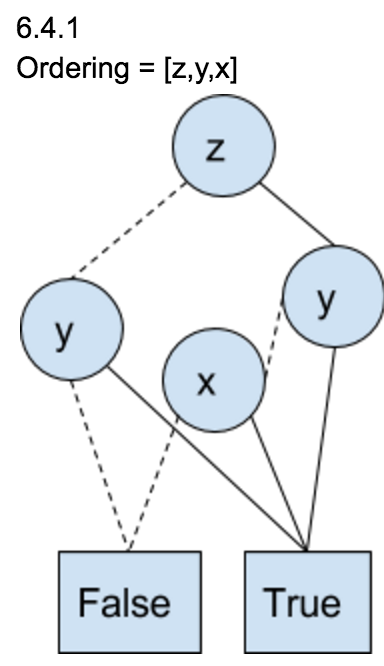
\includegraphics[width=\linewidth]{3a.png}
\endminipage\hfill
\end{figure}
\\b)
\begin{figure}[!htb]
\minipage{0.20\textwidth}
  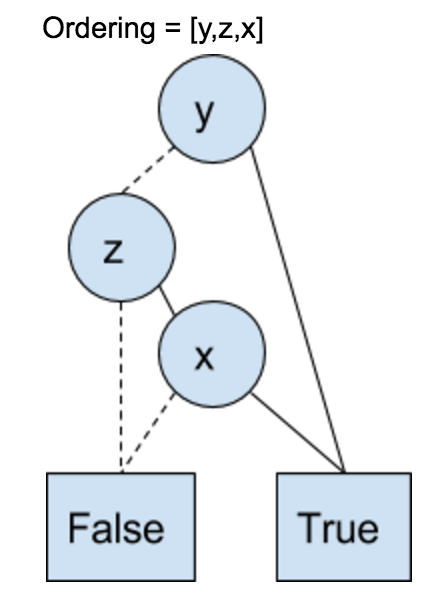
\includegraphics[width=\linewidth]{3b.png}
\endminipage\hfill
\end{figure}
The ordering [y,z,x] has the least number of nodes in it's most reduced form.
\section{Problem 4}
According to theorem 6.7 in the book, all fully reduced OBDD's with the same variables and formulas are equivalent to one other in structure. This follows from the fact that their truth tables are equivalent and if they are both B and $B^`$ are fully reduced and share the same truth tables then it follows that they must be the same OBDD. 
\section{Problem 5}
1) All diagrams are in reduced order, dashes represent the variable is False, and 0 is equivalent to False and 1 is equivalent to 1.
Ordering = [$x_1, x_2$], $\{s_0,s_1\} = (x_1 \land x_2) \lor (x_1 \land \neg x_2)$
\begin{figure}[!htb]
\minipage{0.20\textwidth}
  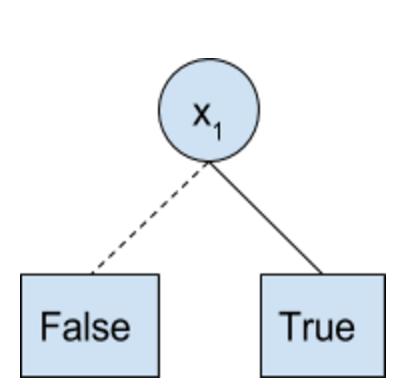
\includegraphics[width=\linewidth]{6a1.png}
\endminipage\hfill
\end{figure}
\\ 
$\{s_0,s_2\} = (x_1 \land x_2) \lor (\neg x_1 \land \neg x_2)$\\
\begin{figure}[!htb]
\minipage{0.20\textwidth}
  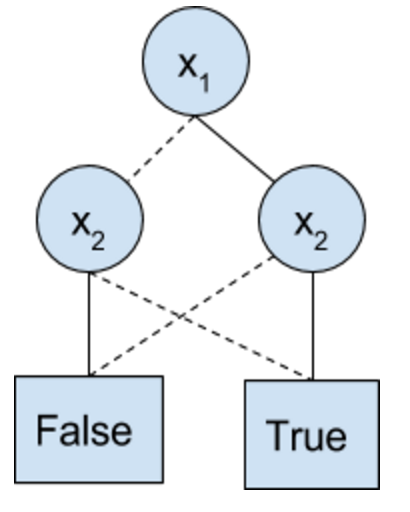
\includegraphics[width=\linewidth]{6a2.png}
\endminipage\hfill
\end{figure} \\
2) \\
Ordering = [$x_1, x_2$], $\{s_0,s_1\} = (x_1 \land \neg x_2) \lor (\neg x_1 \land x_2)$
\begin{figure}[!htb]
\minipage{0.50\textwidth}
  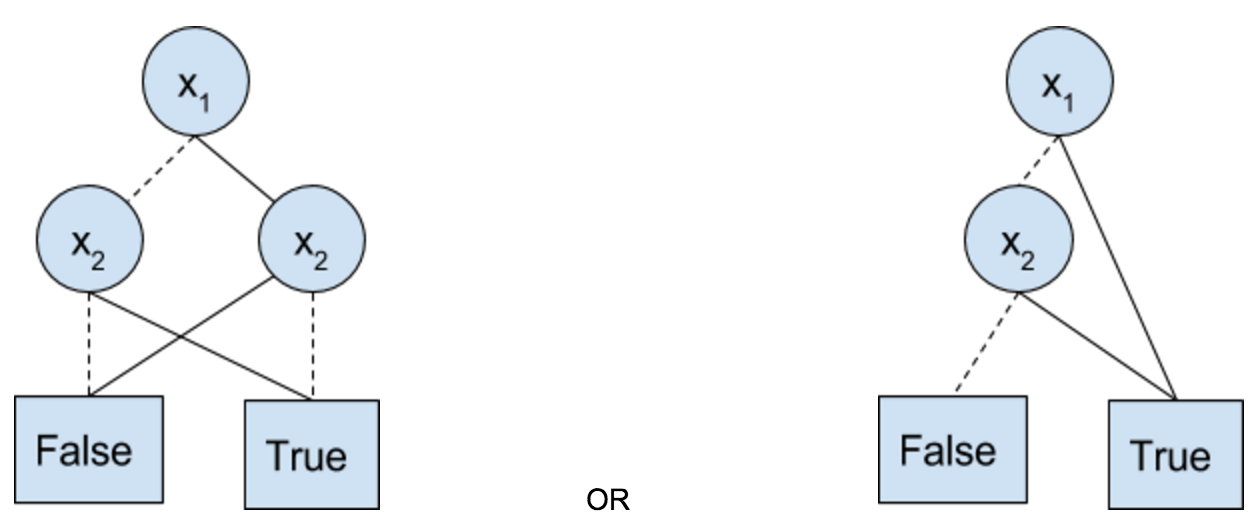
\includegraphics[width=\linewidth]{6b1.png}
\endminipage\hfill
\end{figure}
\\ \\ You can omit the True, True case in the second instance because it isn't possible in our state diagram.\\
\\ $\{s_0,s_2\} = (x_1 \land \neg x_2) \lor (\neg x_1 \land \neg x_2)$ \\
Both of the options available for this state are shown below. The True True case can be eliminated for the same reason as before.
\begin{figure}[!htb]
\minipage{0.20\textwidth}
  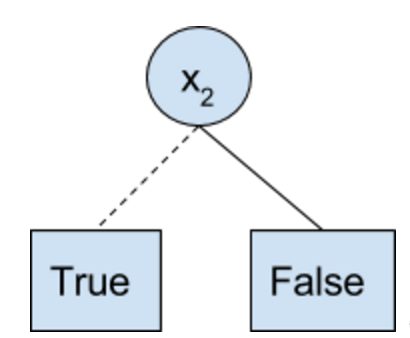
\includegraphics[width=\linewidth]{6b2.png}
\endminipage\hfill
\minipage{0.20\textwidth}
  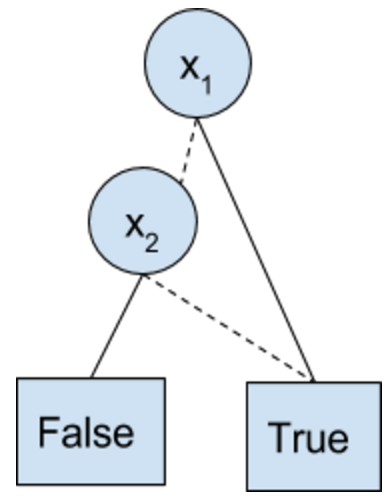
\includegraphics[width=\linewidth]{6b3.png}
\endminipage
\end{figure}

\end{document}